\begin{frame}{Monte Carlo Tree Search(MCTS)}{Quesque le MCTS}
	\begin{block}{}
		\begin{itemize}
			\item Le \textbf{MCTS} est un algorithme de recherche arborescente utilisé pour résoudre des problèmes afin de prendre une décision (un déplacement dans un jeu par exemple).
			\item Il n'utilise pas de fonction d'évaluation heuristique comparé à \textbf{$\alpha$$\beta$} par exemple, et parcours les possibilités aléatoirement, en utilisant les données obtenues précédemment.
			\item Il utilise les méthodes de \textbf{Monte Carlo} pour améliorer son efficacité.
			\item Il possède des variantes, dépendant de leur utilisation, comme celles de \textbf{Coulom}, \textbf{Kocsis} et \textbf{Szepesvari}.
			\item Applicable si toutes les règles de l'application sont connues et si la longueur d'une partie et les gains ont une limite.	
		\end{itemize}
	\end{block}
\end{frame}

\begin{frame}{Monte Carlo Tree Search(MCTS)}{Structure}
	\begin{block}{Arbre de recherche}
		\begin{itemize}
			\item L'arbre de recherche est une \textbf{modélisation} des possibilités de jeu pour la simulation.
			\item Un noeud représente un état du jeu.
			\item Chaque noeud possède deux informations :
			\item\begin{itemize}
				\item - La \textbf{valeur} de sa position.
				\item - Le \textbf{nombre de visites} de ce noeud dans la simulation.
			\end{itemize}
			\item Chaque feuille de cet arbre représente soit un noeud dont les enfants n'ont pas encore été explorés, soit un état final de celui-ci.		
		\end{itemize}
	\end{block}
\end{frame}

\begin{frame}
	\begin{block}{Exemple d'arbre MCTS}
		\begin{center}
			\includegraphics[width=7cm]{ressources/MCTS/tree.png}
		\end{center}
	\end{block}
\end{frame}


\begin{frame}{Monte Carlo Tree Search(MCTS)}{Structure}
    \begin{block}{Plusieurs étapes}
	    	\begin{itemize}
	    		\item 1. Sélection
	    		\item 2. Expansion
	    		\item 3. Simulation
	    		\item 4. Rétropropagation
	    		\item Répété jusqu'à la prise de décision.
	    	\end{itemize}
		\begin{center}
			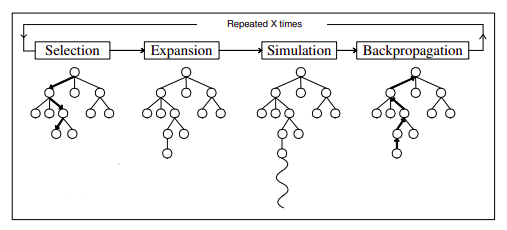
\includegraphics[width=8cm]{ressources/MCTS/MCTSEtapes}
		\end{center}
	\end{block}
\end{frame}

\begin{frame}{Monte Carlo Tree Search(MCTS)}{Sélection}
	\begin{block}{Fonctionnement Sélection}
		\begin{columns}
			\begin{column}{7cm}
				\begin{itemize}
					\item - On commençant à partir de la racine. \item - On applique récursivement une \textbf{stratégie} de sélection pour trouver une feuille de l'arbre à étendre (un chemin qui n'a donc pas encore été exploré).
					\item La stratégie doit, pour optimiser les résultats, faire un consensus entre exploitation et exploration.
					\item Il existe pour cela plusieurs stratégies comme \textbf{OMC}, \textbf{UCT}, \textbf{PBBM}, ...
				\end{itemize}
			\end{column}
			\begin{column}{4cm}
				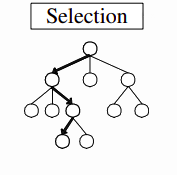
\includegraphics[width=3cm]{ressources/MCTS/Selection.png}
			\end{column}
		\end{columns}
	\end{block}
\end{frame}

\begin{frame}{Monte Carlo Tree Search(MCTS)}{Stratégie Sélection}
	\begin{block}{Stratégie OMC (Objective Monte-Carlo)}
		\begin{itemize}
			\item $U_{i}$ une fonction d'urgence d'un mouvement avec :
			\item $U_{i} = erfc(\frac{v_{0} - v_{i}}{\sqrt{2}\sigma_{i}})$
			\item $v_{0}$ la valeur du meilleur mouvement et $v_{j}$ la valeur du mouvement courant.
			\item $\sigma_{j}$ la déviation de $v_{j}$
			\item $erfc$ la fonction complémentaire d'erreur avec :
			\item $erfc(x) = 1 - \frac{2}{\sqrt{\pi}}\int_{x}^{\infty}e^{-u^{2}}$
			\item La probabilité $P_{m}$ pour chaque $m \in M$ avec :
			\item $P_{m} = \frac{U(m)}{\sum_{j \in S_{i}}^{}U(j)}$
			\item On choisit le prochain mouvement à simuler aléatoirement selon la probabilité $P_{m}$ et peut être longue à calculer.
		\end{itemize}
	\end{block}
\end{frame}

\begin{frame}{Monte Carlo Tree Search(MCTS)}{Stratégie Sélection}
	\begin{block}{PBBM (Probability to be Better than Best Move)}
		\begin{itemize}
			\item Similitude avec la stratégie OMC
			\item $U_{i}$ aussi une fonction d'urgence d'un mouvement avec :
			\item $U_{i} = \exp(-2.4\frac{v_{0} - v_{i}}{\sqrt{2(\sigma_{0}^2 + \sigma_{i}^2)}})) + \epsilon_{i}$
			\item $v_{0}$ la valeur du meilleur mouvement et $v_{i}$ la valeur du mouvement courant.
			\item $\sigma_{0}$ et $\sigma_{i}$ leur déviations.
			\item $\epsilon_ {i}$ une constante assurant que la fonction d'urgence ne soit pas égale à 0 avec :
			\item $\epsilon_ {i} = \frac{0.1 + 2^{-i} + a_{i}}{N}$
			\item $a_{i} = 1$ ou $0$ selon la situation.
		\end{itemize}
	\end{block}
\end{frame}

\begin{frame}{Monte Carlo Tree Search(MCTS)}{Stratégie Sélection}
	\begin{block}{Stratégie UCT (Upper Confidence bounds applied to Trees)}
		\begin{itemize}
			\item La stratégie UCT sélectionne un noeud $k$ fils du noeud $p$ qui satisfait la formule suivante :
			$$k \in argmax_{i\in I}(v_{i} + C \times \sqrt{\frac{\ln n_{p}}{n_{i}}})$$
			\item $I$ un set de noeuds atteignable par le noeud $p$.
			\item $v_{i}$ la valeur du noeud $i$
			\item $n_{p}$ et $n_{p}$ le nombre de fois que les noeuds $p$ et $i$ on été visités.
			\item $C$ une constante.
			\item Facile à implémenter et beaucoup utilisée.
		\end{itemize}
	\end{block}
\end{frame}

\begin{frame}{Monte Carlo Tree Search(MCTS)}{Stratégie Sélection}
	\begin{block}{Stratégie UCB1-TUNED}
		\begin{itemize}
			\item Variante de la stratégie UCT
			\item Cette sélectionne un noeud $k$ fils du noeud $p$ qui satisfait la formule suivante :
			$$k \in argmax_{i\in I}(v_{i} + C \times \sqrt{\frac{\ln n_{p}}{n_{i}}\times \min(\frac{1}{4}, V_{i}(n_{i}))})$$
			\item avec $V_{i}$ une estimation de la borne supérieur de la variance de $v_{i}$ avec comme formule :
			$$V_{i}(n_{i}) = (\frac{1}{n_{i}}\sum_{t=1}^{n_{i}}R_{i,t,j}^2 - v_{i}^2 + \sqrt{\frac{2\ln n_{p}}{n_{i}}})$$
			\item $R_{i,t,k}$ la $t$-ième récompense obtenu au noeud $i$ pour le joueur $j$
		\end{itemize}
	\end{block}
\end{frame}

\begin{frame}{Monte Carlo Tree Search(MCTS)}{Expansion}
	\begin{block}{Fonctionnement Expansion}
		\begin{columns}
			\begin{column}{8cm}
				\begin{itemize}
					\item Dépend des règles du jeu.
					\item \textbf{Crée} un noeud à partir du noeud sélectionné si celui-ci n'est pas final.
					\item On ne peut pas garder tout les résultats en mémoire.
					\item Il existe plusieurs stratégies pour choisir les noeuds à garder.
				\end{itemize}
			\end{column}
			\begin{column}{4cm}
				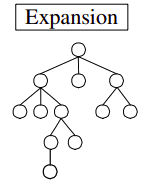
\includegraphics[width=3cm]{ressources/MCTS/Expansion.png}
			\end{column}
		\end{columns}
	\end{block}
\end{frame}

\begin{frame}{Monte Carlo Tree Search(MCTS)}{Stratégie Expansion}
	\begin{block}{Exemple de statégies d'expansion}
			\begin{itemize}
				\item - Garder seulement un noeud par jeu simulé. Ce noeud correspond à la première position qui n'étaient pas déjà stockées lors d'un parcours.
				\item - Continuer à stocker les enfants d'un noeuds jusqu'à un nombre limité de simulations (nécessite une quantité conséquente de mémoire)
			\end{itemize}
	\end{block}
\end{frame}

\begin{frame}{Monte Carlo Tree Search(MCTS)}{Simulation}
	\begin{block}{Fonctionnement Simulation}
		\begin{columns}
			\begin{column}{7cm}
				\begin{itemize}
					\item - Réalise une \textbf{simulation} d'une partie aléatoirement (ou partiellement) à partir du noeud étendu
					\item - Continue de parcourir des états de jeux jusqu'à atteindre un état \textbf{final}, afin d'obtenir un résultat.
					\item Il existe des stratégies de simulation, difficiles à définir car on doit garder un bon compromis entre recherche et exploitation.
					\item Ces stratégies peuvent utiliser des connaissances du jeu (patterns, considérations, ...)
				\end{itemize}
			\end{column}
			\begin{column}{4cm}
				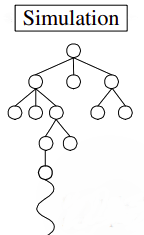
\includegraphics[width=3cm]{ressources/MCTS/Simulation.png}
			\end{column}
		\end{columns}
	\end{block}
\end{frame}

\begin{frame}{Monte Carlo Tree Search(MCTS)}{Stratégie Simulation}
	\begin{block}{Exemple d'une stratégie : Sequence-like Simulation}
		\begin{columns}
			\begin{column}{8cm}
				\begin{itemize}
					\item Cette stratégie est adapté au jeu de GO, et consiste à :
					\item - \textbf{Sélection} de chaque coup à proximité du dernier coup joué $c_{0}$ avec $E$ l'ensemble des coups adjacents. 
					\item - \textbf{Choix} du coup à jouer dans $E$, en cherchant des motifs de jeu de taille 3x3 à une distance 1 de Manhattan avec $c_{0}$. 
					\item - Si plusieurs motifs correspondent : choix aléatoire du motif parmi eux en jouant au milieu de celui-ci.
					\item - Si aucun est reconnu, choix aléatoire.
				\end{itemize}
			\end{column}
			\begin{column}{3cm}
				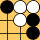
\includegraphics[width=2cm]{ressources/MCTS/3x3GridGo.png}
				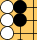
\includegraphics[width=2cm]{ressources/MCTS/3x3GridGo2.png}
			\end{column}
		\end{columns}
	\end{block}\end{frame}

\begin{frame}{Monte Carlo Tree Search(MCTS)}{Rétropropagation}
	\begin{block}{Fonctionnement de la rétropropagation}
		\begin{columns}
			\begin{column}{8cm}
				\begin{itemize}
					\item - Utilise le résultat de la simulation pour \textbf{propager} l'information aux \textbf{parents} de ce noeud récursivement.
					\item - Se propage jusqu'au noeud le plus haut afin de mettre les données de tout les noeuds  à jour.
					\item - Change alors la valeur des noeud 
					par une souhaité et garde en mémoire sa visite.
					\item  Pour intérpréter, on pose $R_{i}$ le résultat d'une partie (de GO par exemple) :
					
					- $R_{i} = +1$ si l'IA gagne
					
					- $R_{i} = -1$ si l'IA perd
					
					- $R_{i} = 0$ si égalité.
				\end{itemize}
			\end{column}
			\begin{column}{4cm}
				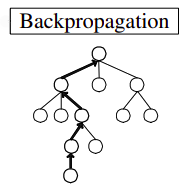
\includegraphics[width=3cm]{ressources/MCTS/Backpropagation.png}
			\end{column}
		\end{columns}
	\end{block}
\end{frame}

\begin{frame}{Monte Carlo Tree Search(MCTS)}{Stratégie Rétropropagation}
	\begin{block}{Exemple de stratégies}
		\begin{itemize}
			\item Il existe aussi plusieurs stratégies de rétropropagation :
			\item \textbf{Moyenne} : Prend la moyenne des résultats : $v_{i} = \frac{\sum_{i}^{}R_{i}}{n_{i}}$ avec $v_{i}$ la valeur du noeud et $n_i$ le nombre de fois qu'il a été visité.
			\item \textbf{Max} : Prend le max des résultats des enfants (pas efficace)
			\item \textbf{Moyenne informée} : Attribue de plus grande valeur aux meilleurs résultats afin d'avoir le meilleurs résultats plus rapidement.
			On a : $v_{i} = \frac{\sum_{j}^{}(v_{j}\times n_{j}\times U_{j})}{\sum_{j}^{}(n_{j}\times U_{j})}$ avec $U_{j}$ la fonction d'urgence utilisé pour la stratégie de sélection OMC.
			\item \
			\item Mais la majorité des programmes utilise la stratégie \textbf{Moyenne} car elle donne de meilleurs résultats.
		\end{itemize}
	\end{block}
\end{frame}

\begin{frame}{Monte Carlo Tree Search(MCTS)}{Choix du mouvement final}
	\begin{block}{Exemple de choix du mouvement}
		\begin{itemize}
			\item \textbf{Maximum des noeuds}: On prend le noeud qui a la plus grande valeur.
			\item \textbf{Noeud le plus robuste}: On prend le noeud qui a été visité le plus de fois.
			\item \textbf{Mix}: On prend le noeud qui est à la fois le maximum et le plus robuste (on fait des simulations jusqu'à en obtenir un si non existant)
			\item \textbf{Noeud le plus sécurisé}: On prend le noeud qui maximise une borne de confiance (a besoin d'expérimentation).
			\item Il n'y pas beaucoup de différence parmi ces choix, sauf lorsque le temps pour faire le choix est faible, où le choix max devient moins efficace.
		\end{itemize}
	\end{block}
\end{frame}

\begin{frame}{Monte Carlo Tree Search(MCTS)}{Application}
	\begin{block}{Exemple d'applications}
		\begin{itemize}
			\item Pour les jeux à deux joueurs comme pour le GO, le \textbf{MCTS} a été une révolution :
			\item Le programme MCTS \textbf{Mogo Titan} a permis pour la première fois de battre un joeurs pro de Go avec contrainte (7 pierres d'handicap).
			\item Utilisés par les programmes \textbf{MOGO}, \textbf{CRAZY STONE}, \textbf{FUEGO}, ... qui sont aussi très efficace.
			\item \textbf{AlphaGo} utilise aussi le MCTS pour sa recherche de coup (en l'adaptant à son programme).
			
		\end{itemize}
	\end{block}
\end{frame}